\chapter{Moodle plug-in készítés folyamata}

\section{Előzetes ötletek, első lépések}

Első körben érdemes definiálni, hogy mit kell tudnia a pluginnek és így milyen fajta pluginre lesz szükség. Tudjon
\begin{itemize}
    \item Feladat nehézségeket kiválasztani,
    \item Feladat nehézség szerint tudjon feladatot generálni,
    \item A felhasználótól tudjon lekérni megoldást,
    \item A feladat megoldását összevetve a felhasználó megoldásával tudja megjeleníteni.
\end{itemize}

Ehhez nem szükséges speciálisabb plugint kiválasztani, elég, ha local. Ezután alkossuk meg a kötelező fájlokat. A lang\_en\_local\_szakdolgozat első sorába írjuk be az alábbi sort:

\begin{lstlisting}[language=php]
$string['pluginname'] = 'Normalization';
\end{lstlisting}

Ezzel kész is fejléc címe. Ezután hozzuk létre a version.php-t, amelybe az alábbi sorokat tegyük:

\begin{lstlisting}[language=php]
$plugin->component = 'local_szakdolgozat';
$plugin->version = 2021013000;
\end{lstlisting}

És már csak indítsuk újra a Moodle-t, ekkor felismeri a plugint és feltelepíti. Ezután pedig készítsük el az index.php-t, a classes mappát és a mappába másoljuk be a Relációsémákat generáló és megoldó osztályokat.

\section{A plugin felépítése}

A pluginnak 4 része lesz:
\begin{enumerate}\setcounter{enumi}{-1}
    \item Fejléc megalkotása
    \item Nehézség kiválasztása
    \item Feladat generálása
    \item Megoldás megjelenítése
\end{enumerate}

Elsőnek beállítjuk az url-t, a címet,a kapcsolódását a moodle-hez, a fejléc szövegét, és milyen kialakítású legyen.
Ezenkívül meghívjuk a saját osztályainkat, illetve a gyökérkönyvtárban lévő config.php-t, mivel szükségünk lesz a \$PAGE, illetve a \$OUTPUT változókra. 
\begin{lstlisting}
<?php

require(__DIR__. '/../../config.php');
require_once('classes/Relaciosema.php');

$PAGE->set_url(new moodle_url('/local/szakdolgozat/index.php'));
$PAGE->set_context(context_system::instance());
$PAGE->set_title(get_string('pluginname', 'local_szakdolgozat'));
$PAGE->set_heading(get_string('heading', 'local_szakdolgozat'));
$PAGE->set_pagelayout('standard');

echo $OUTPUT->header();
?>
\end{lstlisting}

A nehézség kiválasztása egy egyszerű nyomógombos megoldás, kezdeti értéknek az egyszerű megadva. Amelyiket kiválasztja a felhasználó, arról fog kapni egy feladatot. A nehézség mentése az urlben történik és egy \$difficulty változóval történik a kiolvasása. \par

A Feladat generálása előtt egy felirat található, ahol egy leírás található, hogy milyen formában kell beküldeni a megoldást. Ez azért fontos, hogyha egy megoldást és egy felhasználói választ akarunk összeegyeztetni, akkor elsőnek érdemes átalakítani egy felhasználói választ egy Relációséma példánnyá, így könnyebben tudjuk kezelni. A feladat generálás után pedig elmentjük, illetve bekérjük a felhasználótól az általa gondolt jó választ. Ha ez megtörtént, akkor a megadott válaszokat a \textbf{2NF}, \textbf{3NF} és \textbf{BCNF} változókban mentjük és ugrunk a megoldás megmutatására.\par

A legutolsó oldalon pedig a feladaton kívül láthatjuk az általunk megadott választ és a megoldást. Ezután tudunk másik nehézséget választani vagy ebből a nehézségből egy új feladatot kérni. A plugin nem tudja kiértékelni a felhasználó által megadott megoldással, de ez nincs is a feladatkiírásban, így nem probléma. \par

\section{Képernyőképek}

Magyar nyelvű felület:

\begin{center}
    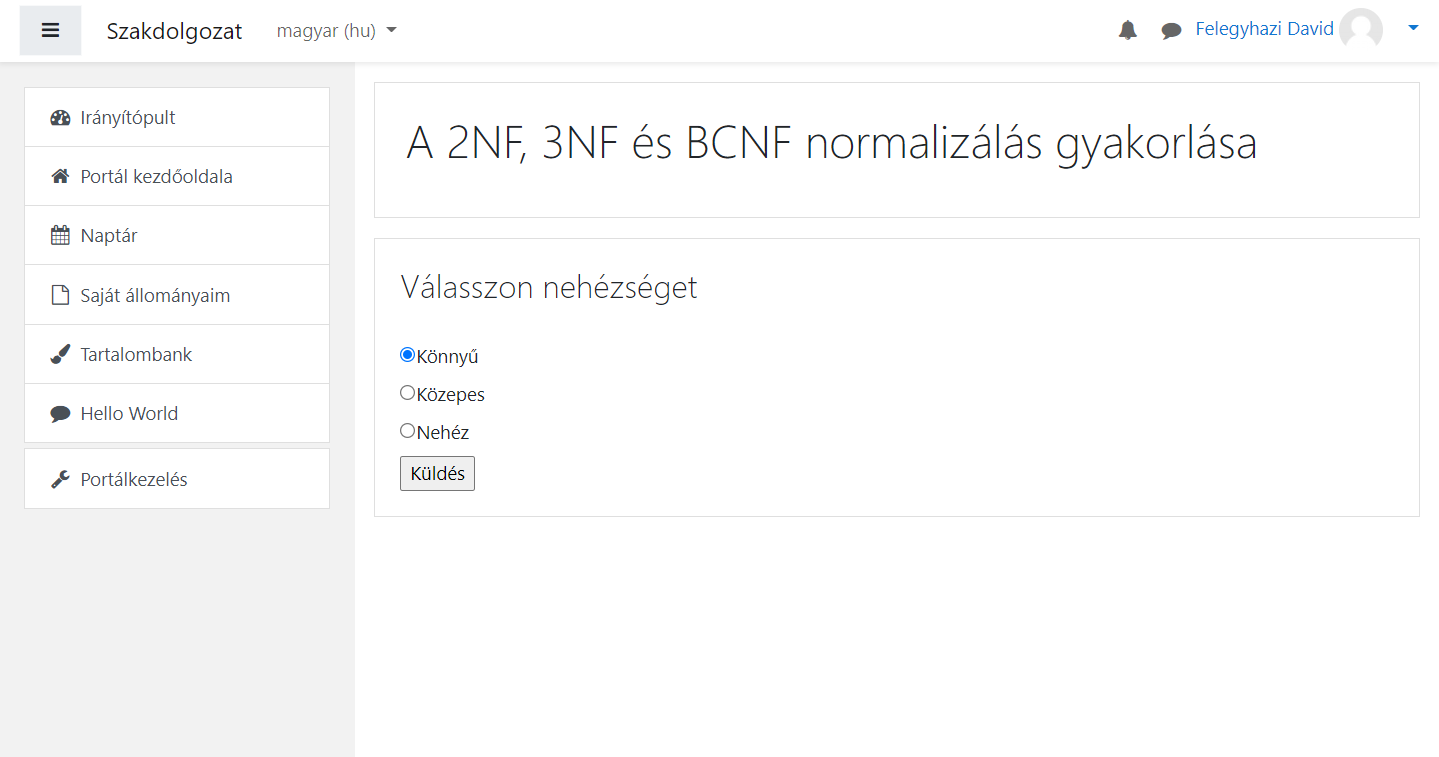
\includegraphics[scale=0.4]{Fejezetek/Images/magyar01.png}
    \hfill \break
    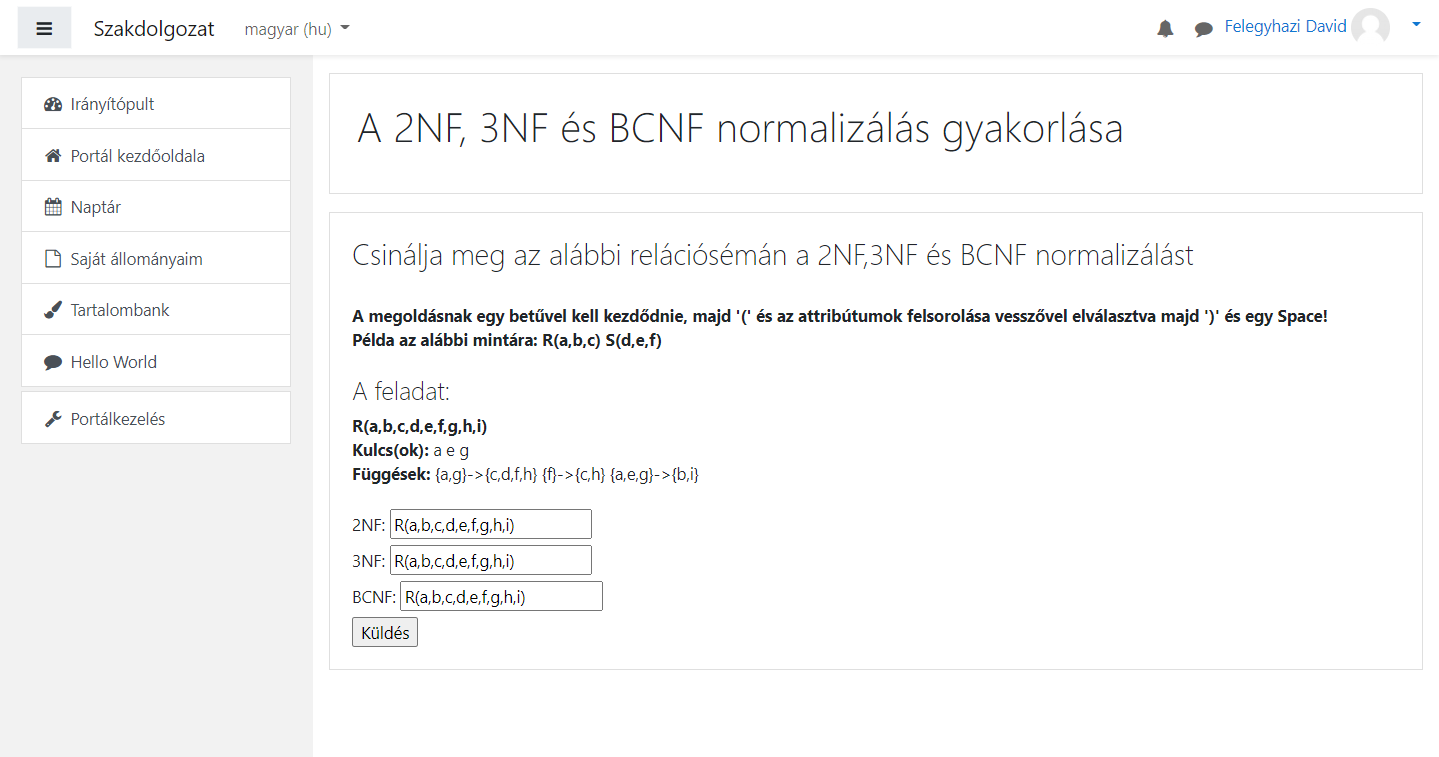
\includegraphics[scale=0.4]{Fejezetek/Images/magyar02.png}
    \hfill \break
    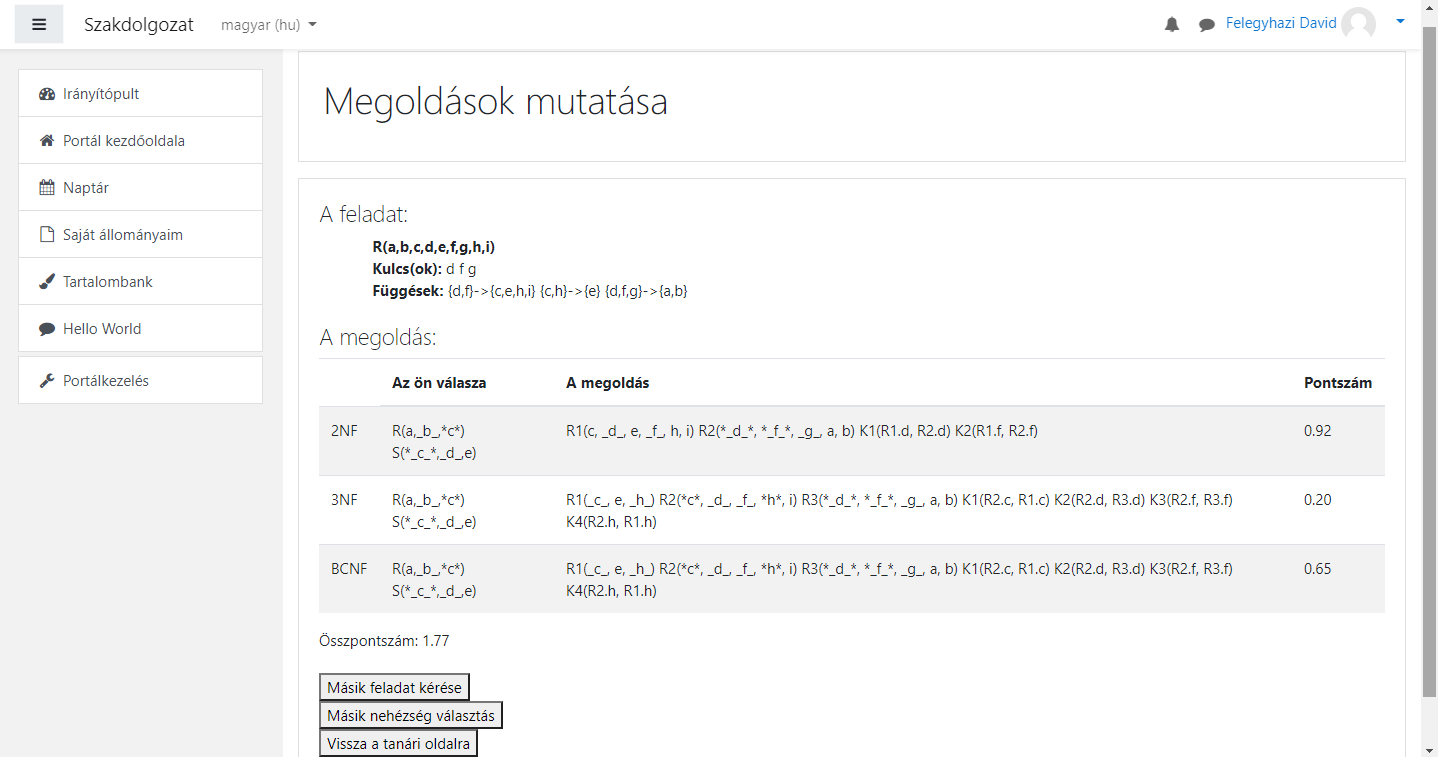
\includegraphics[scale=0.4]{Fejezetek/Images/magyar03.png}
\end{center}

Angol nyelvű felület:

\begin{center}
    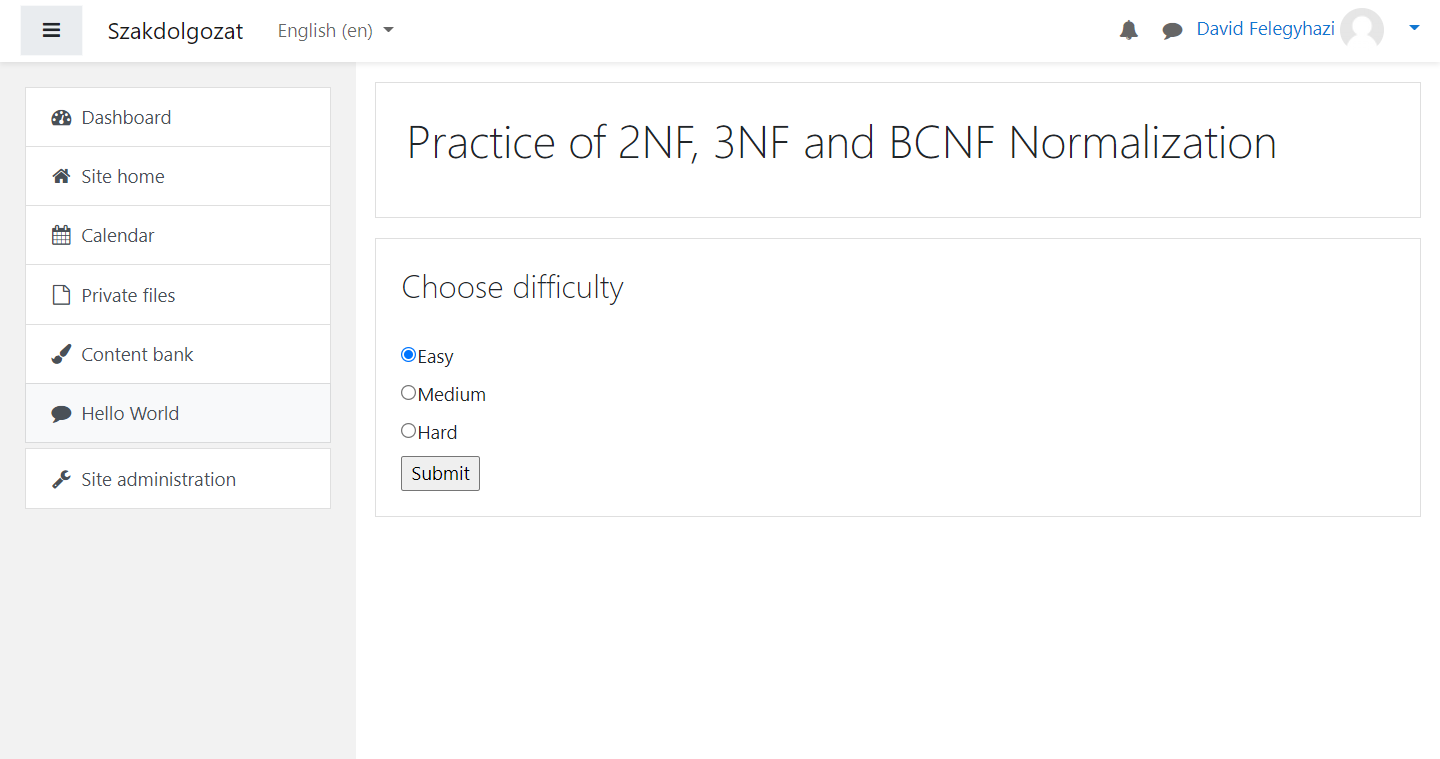
\includegraphics[scale=0.4]{Fejezetek/Images/english01.png}
    \hfill \break
    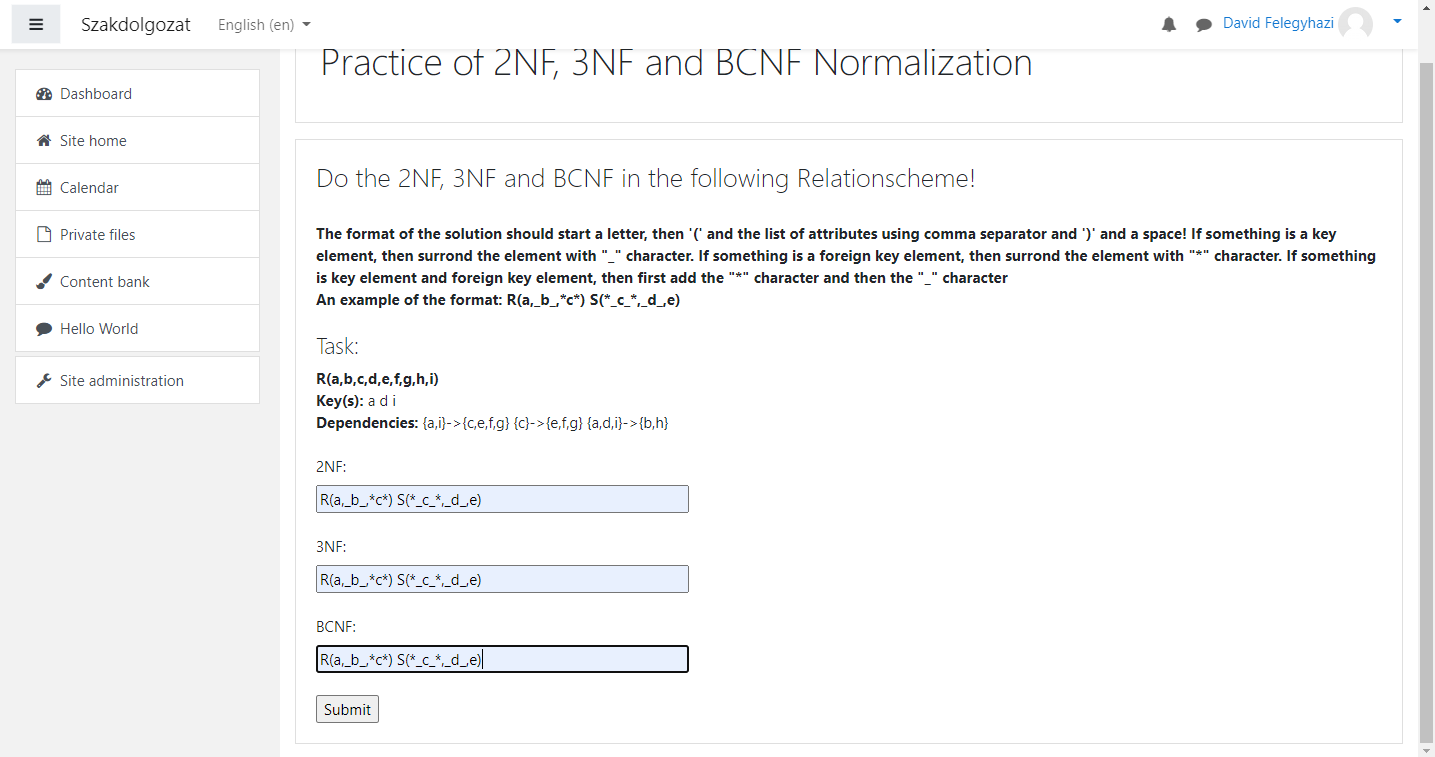
\includegraphics[scale=0.4]{Fejezetek/Images/english02.png}
    \hfill \break
    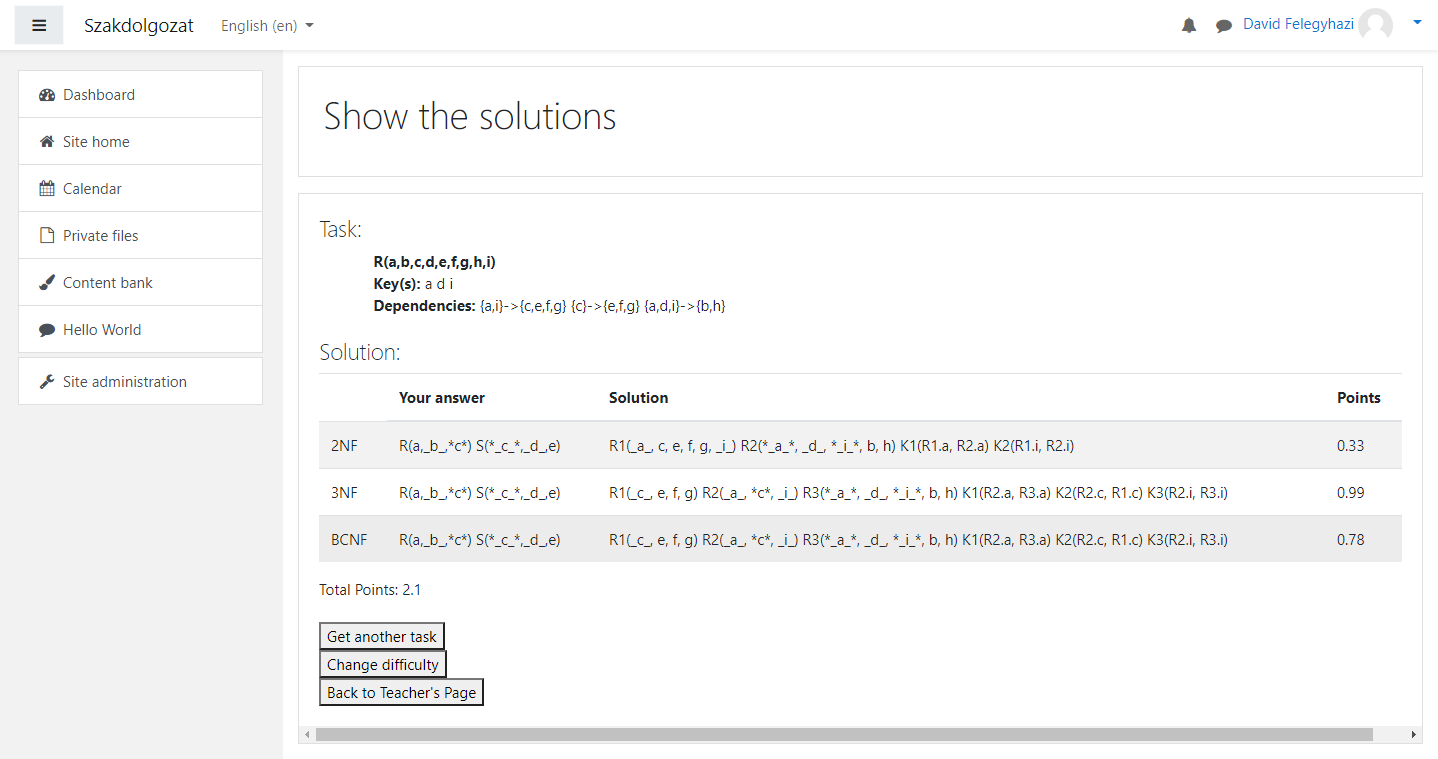
\includegraphics[scale=0.4]{Fejezetek/Images/english03.png}
\end{center}